\documentclass[11pt]{article}
\usepackage[utf8]{inputenc}
\usepackage{fullpage}
\usepackage{graphicx}
\usepackage{booktabs}
\usepackage{setspace}
\usepackage{bm}
\usepackage[font={bf}]{caption}
\usepackage{subcaption}
\usepackage{pdfpages}
\setlength{\parindent}{0em}
\setlength{\parskip}{0.6em}
\usepackage[numbers,sort&compress]{natbib}
\usepackage{hyperref}
\usepackage{amsmath}
\usepackage{natbib}   % omit 'round' option if you prefer square brackets
\bibliographystyle{plainnat}
\usepackage{chngcntr}
\usepackage{ amssymb }

% ----- Figures and tables ----- 
\newcommand{\tabincell}[2]{\begin{tabular}{@{}#1@{}}#2\end{tabular}}
\usepackage{fancyhdr}
\usepackage[labelfont=bf]{caption} % bold text for captions
\usepackage[para]{threeparttable} % fancy tables, check these before you use them
\usepackage{url}
\usepackage{makecell}
\usepackage{hhline}
\usepackage{multirow}

\usepackage{amsthm}
\newtheorem*{remark}{Remark}

\onehalfspacing

\title{\textbf{Statistical Consulting Report} \\
\large Restricted Entry: Is bias limiting Sikhs’ access to mental health services?}
\author{Consultant: Ning Shen \\
Clients: Maria Stahre, Rajeena Kumar}
\date{}

\begin{document}
\maketitle

\begin{abstract}
    Studies have shown that in North America Racial/Ethnic (RE) disparities  exist among social service providers when providing social services to minority groups \citep*{Kugelmass2016,Shin2016}. Researchers of this  study aim to investigate  RE bias within the population of  counsellors in the province of British Columbia towards Punjabi Sikh individuals in terms of how receptive the service provider is to provide social services. In this statistical report, logistic regression and ordinal regression are proposed for the two response variables related to responsiveness and reception rate respectively. Potential confounding factors for one of the predictors are also discussed. Furthermore, a power analysis is included so that the researchers may decide a proper sample size for the upcoming experiment.
\end{abstract}


\section{Introduction}
Research has identified RE disparities in  delivery of social services such as  counselling in North America. Literatures review of RE biases has found that counselling service providers seem  to have an implicit bias, that is,  a positive attitude towards Caucasians and a negative attitude towards people of color \citep*{Kugelmass2016,Shin2016}. This  study aims to investigate RE bias at the entry point of social services. Specifically, the study seeks to examine the possibility of RE disparities in accessing mental health services  by a particular South Asian (SA) group of individuals (i.e., Punjabi Sikh individuals) in  Canada. The main interest  is  the service providers’ possible bias towards  religious individuals of Sikh background in terms of the service providers’ receptiveness to the service recipients.  The secondary objective is to investigate  the impact of other factors such as gender, accent and/or intergroup contact on the accessibility of the services.

\section{Study Description}
TThe participants of  this study will be randomly selected social service providers, i.e.,  counsellors,  from professional associations or licensure bodies common to BC as found on their public directories.  Participants will receive a standardized (i.e., pre-recorded) voicemail representing one of the conditions regarding the status of religion, gender and/or accent through random assignment. A pilot study has identified that certain Sikh names and Christian names are highly likely to conjure up an image of a Sikh or Christian person, respectively. An assumption is thus made that the participants are able to identify  the religion of the caller by his/her name. In terms of intergroup contact, the experiment will be performed on psychological counsellors from two cities with distinct percentage of Punjabi Sikh individuals. To reduce the possibility that the phone call will be answered, all calls will be placed after regular working hours (e.g., 8:30 pm). A pilot experiment with 20 participants will be conducted to determine the sample size required to obtain a power of 0.8 due to the scarcity of research in this area. Whether the service provider returns the phone message and offers appointments will be recorded as response variables. An example of all possible variables is shown in \autoref{tab:vars}. In the real dataset, columns will be variables in \autoref{tab:vars} and rows will be phone messages. 

One thing in particular to note is that, variable \textit{city} is included in the analysis as one of the predictors instead of the level of intergroup contact because of the potential confounding factors, such as demographic characteristics of the participants in different cities. In other words, participants in one city are less prejudiced towards Sikh patients not necessarily because of a higher intergroup contact, but also possibly because of a higher proportion of Sikh councellors in that city. Therefore, we could only make inference on the \textit{city} factor through the analysis rather than the factor of intergroup contact. To infer the causal relationships between RE disparities and level of intergroup contact, further investigation beyond the scope of this study is needed.

\hspace*{-4cm}
\begin{table}[!h]
    \centering
    \begin{tabular}{ |c|c|c| }
    \hline
     \textbf{Variable Type} &  \textbf{Variable Name}  & \textbf{Possible Values} \\
     \hline
     \multirow{4}{*}{\tabincell{c}{Predictors / \\ independent variables}} & \textit{religion} &  `Sikh' or `Non-Sikh' \\ 
     \cline{2-3}
     & \textit{gender} & `Male' or `Female' \\ 
     \cline{2-3}
     & \textit{accent} & `Present' or `Absent' \\ 
     \cline{2-3}
      & \textit{city} & `Richmond' or `Surrey'\\
      \cline{2-3}
     \hline
     \multirow{2}{*}{\tabincell{c}{Responses / \\ dependent variables}} & \textit{callback} &  `True' (coded as `1') or `False' (coded as `0') \\ 
     \cline{2-3}
     & \textit{appoint\_offer} & `Yes', `Not sure' or `No' (coded as `2', `1', `0' respectively) \\ 
     \hline
    \end{tabular}
    \caption{Example table of variables included in the analysis.}
    \label{tab:vars}
\end{table}


\section{Proposed Statistical Analysis}
Since the project is only at its early stage with no data available, simulated data are generated for a clear presentation of the proposed analysis under the assumption that the data structure and possible values in \autoref{tab:vars} are correct. A logistic regression model is proposed for the response coded as a binary variable (i.e., \textit{callback}). An ordinal regression model, which is an extension of the logistic regression model, is recommended for the case where the response is coded as an ordinal variable with more than two levels. Specifically, an ordinal variable is a variable whose value exists on an arbitrary scale where only the relative ordering between different values is important, such as \textit{appoint\_offer}. A sample analysis though statistical programme language \texttt{R} is illustrated below as well as interpretation for the results. In the following analysis we include all predictors from \autoref{tab:vars}, but choice of the predictors is flexible due to nature of the models. Researchers of the study may choose a desired set of predictors depending on the circumstances. All programming codes can be found in my \href{https://github.com/NingShen1997/STAT551_Case34}{Github repository}.


\begin{figure}[!b]
    \centering
    \begin{subfigure}{0.45\textwidth}
        \centering
        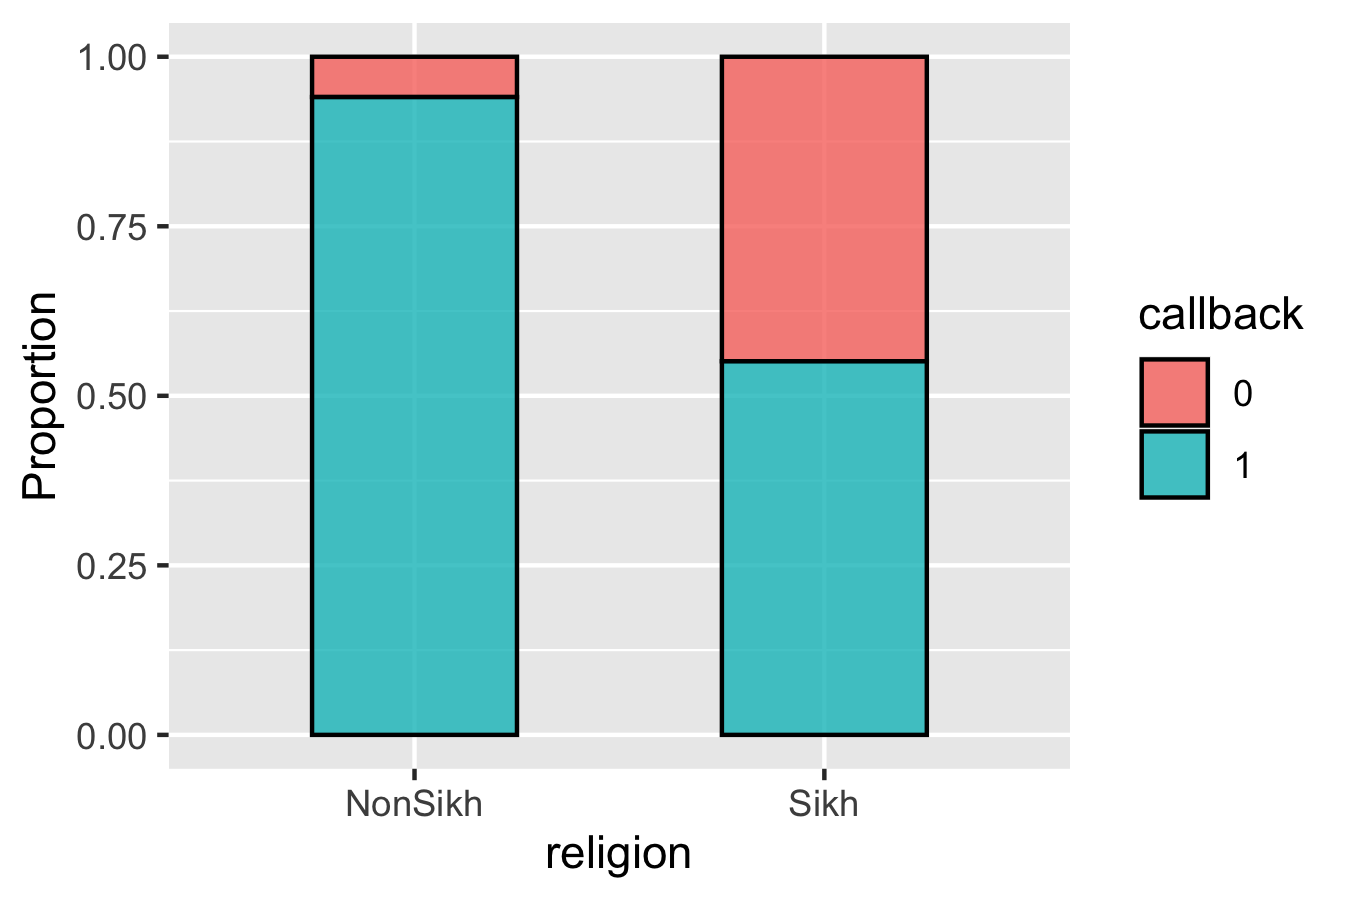
\includegraphics[width=\textwidth]{../../Plots/Proportions_callback_religion.png}
        \caption{}
    \end{subfigure}
    \begin{subfigure}{0.45\textwidth}
        \centering
        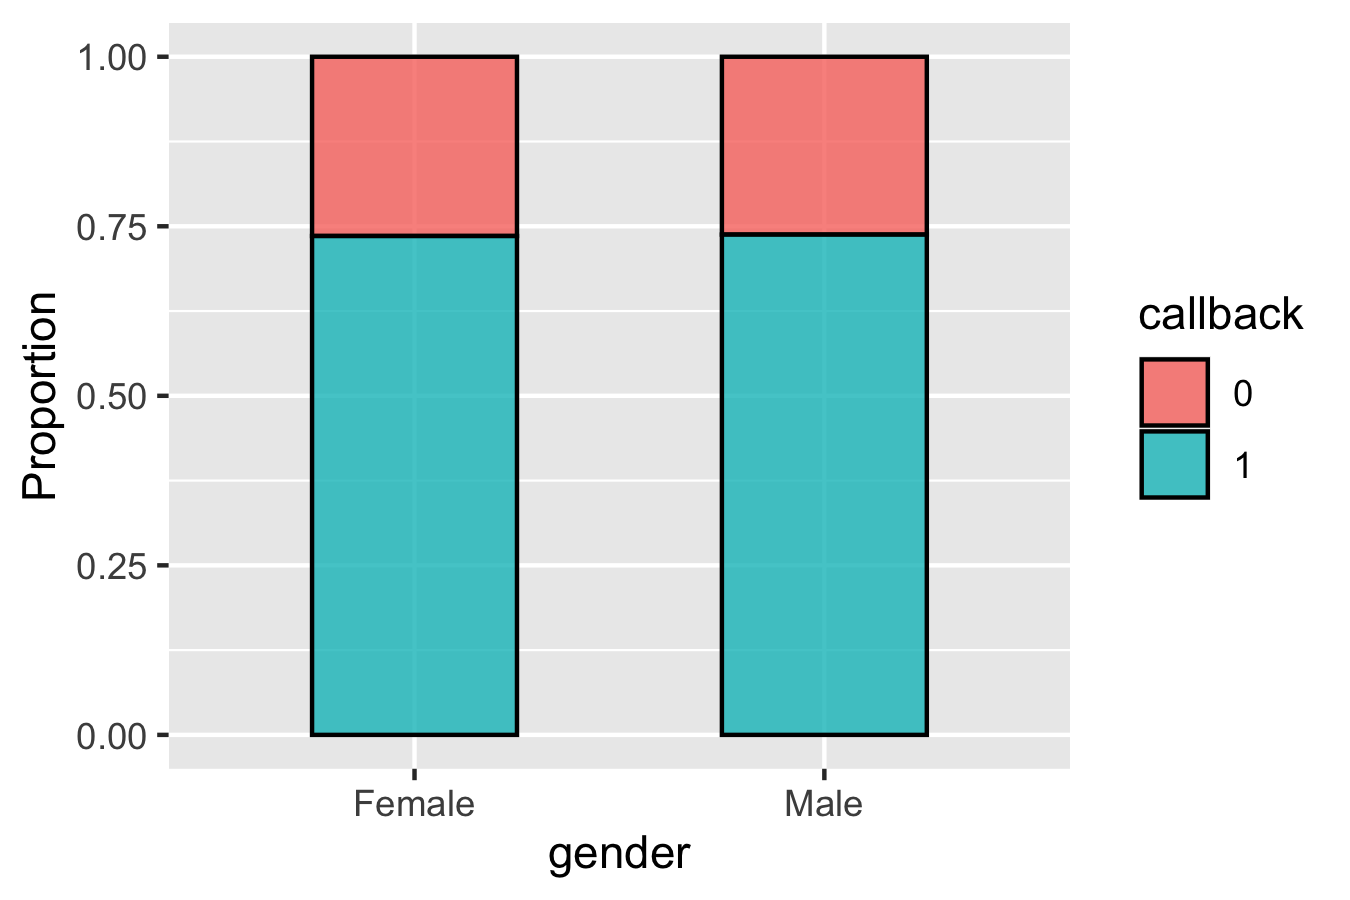
\includegraphics[width=\textwidth]{../../Plots/Proportions_callback_gender.png}
        \caption{}
    \end{subfigure}
    \begin{subfigure}{0.45\textwidth}
        \centering
        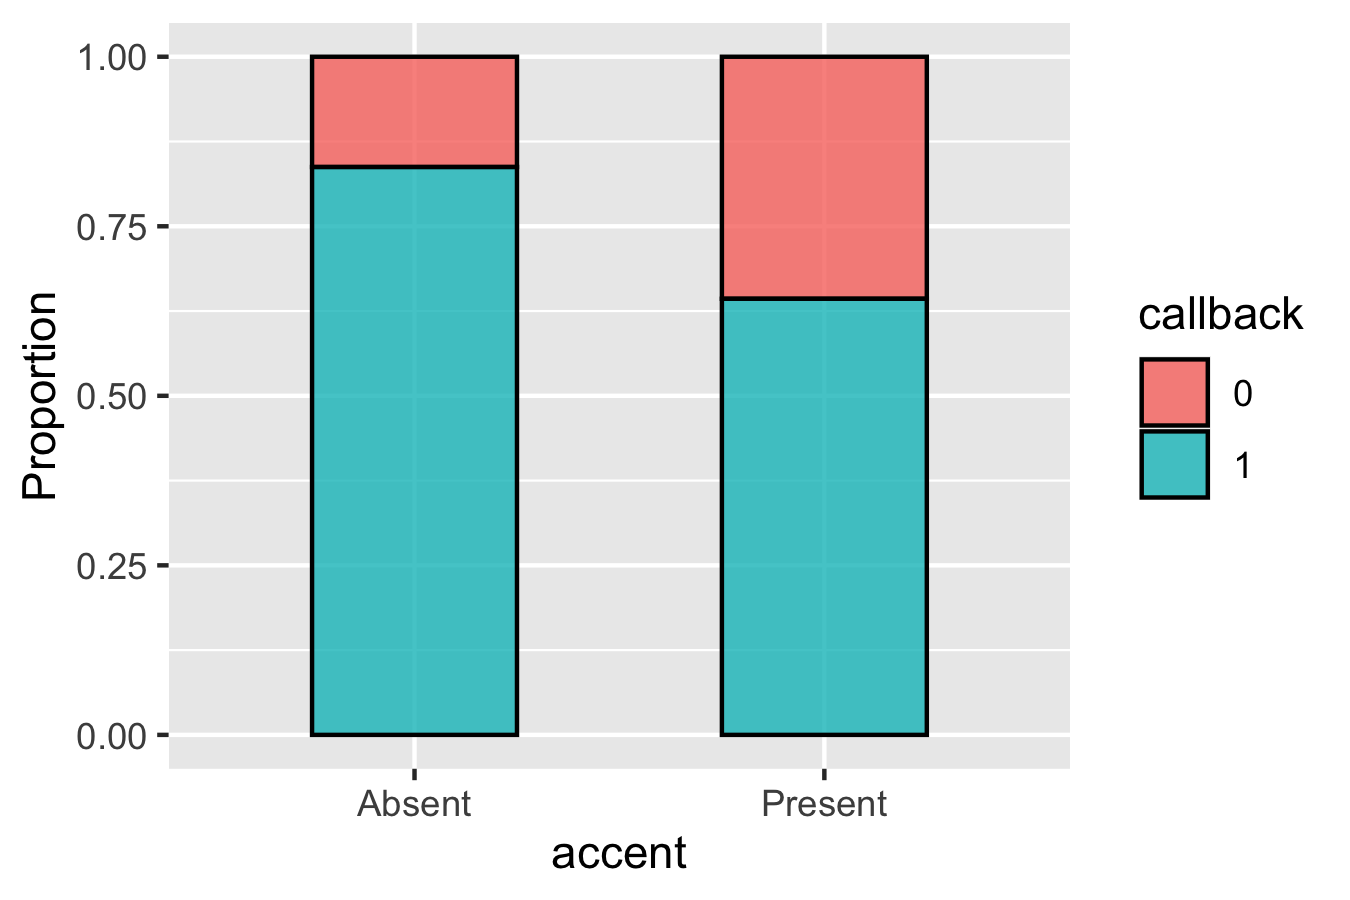
\includegraphics[width=\textwidth]{../../Plots/Proportions_callback_accent.png}
        \caption{}
    \end{subfigure}
    \begin{subfigure}{0.45\textwidth}
        \centering
        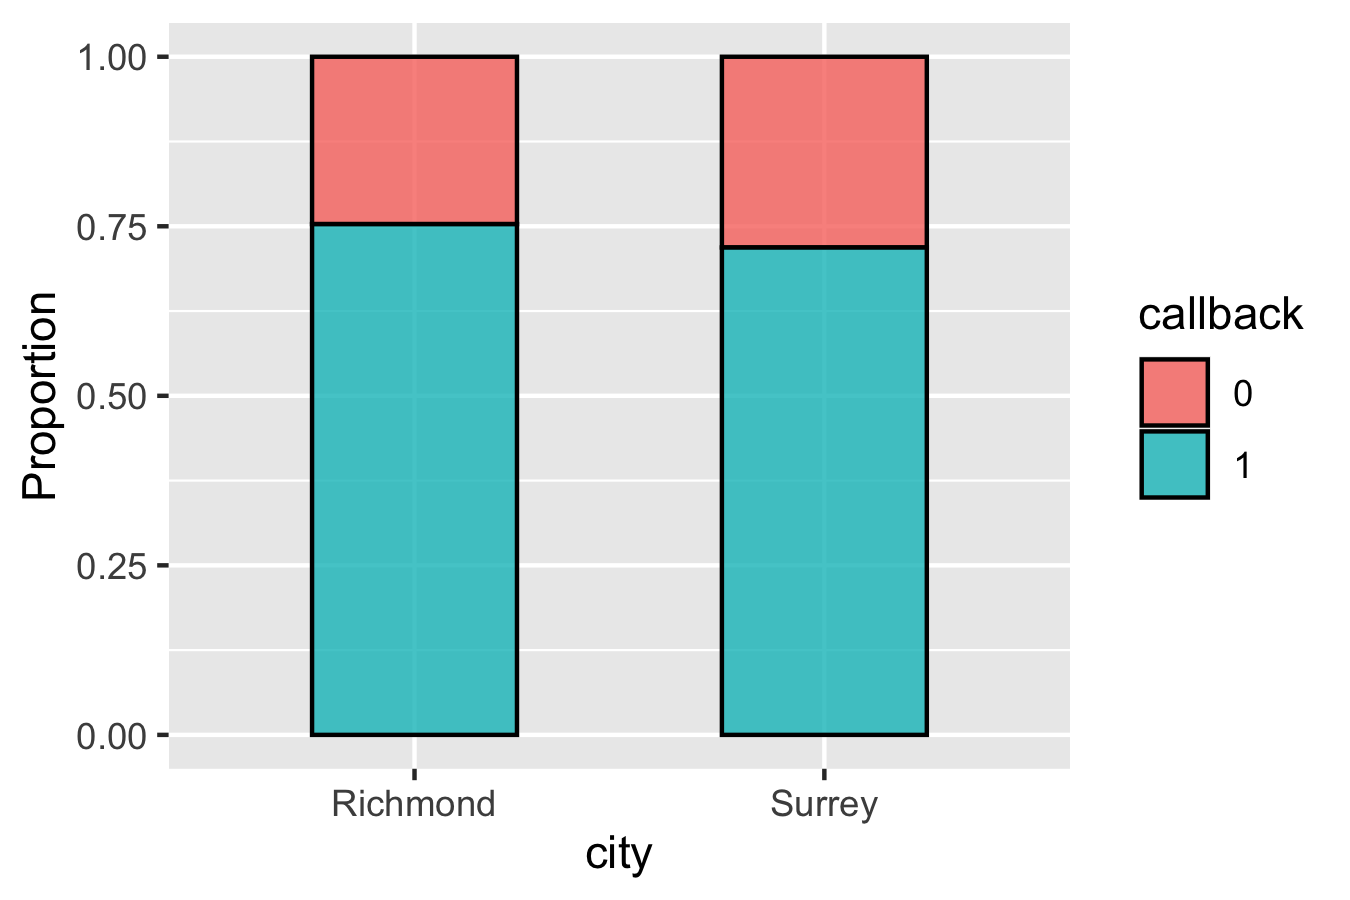
\includegraphics[width=\textwidth]{../../Plots/Proportions_callback_city.png}
        \caption{}
    \end{subfigure}
    \caption{Distribution of \textit{callback} in predictors a) \textit{religion}, b) \textit{gender}, c) \textit{accent} and d) \textit{city}.}
    \label{fig:eda1}
\end{figure}





\subsection{Logistic regression on \textit{callback}}
\label{sec:logit}

As an exploratory plot, \autoref{fig:eda1} depicts the distribution of \textit{callback} within possible values of the predictors respectively. \textit{Religion} and \textit{accent} are the two factors that have distinctive proportions of `no callback' in different categories, while \textit{gender} and \textit{city} seem to have little influence on the callback rate. Further, we use interaction plots to determine if any possible interaction terms should be included in the model. \autoref{fig:interact} is an example of the interaction plot between predictors \textit{religion} and \textit{accent}. The plot shows that the slopes of the lines are pretty close, i.e. the decrease of callback rate from `non-Sikh' to `Sikh' does not differ by the status of \textit{accent}, thus no interaction term is needed between \textit{religion} and \textit{accent} in the regression model. We also provide two simulated situations in the Appendix \autoref{fig:interact2}, where the slopes of the lines differ drastically, indicating the two predictors have interaction effect present. Examination of interactions between every pair of predictors shall be done by the researchers before fitting the model.

\begin{figure}[!h]
    \centering
    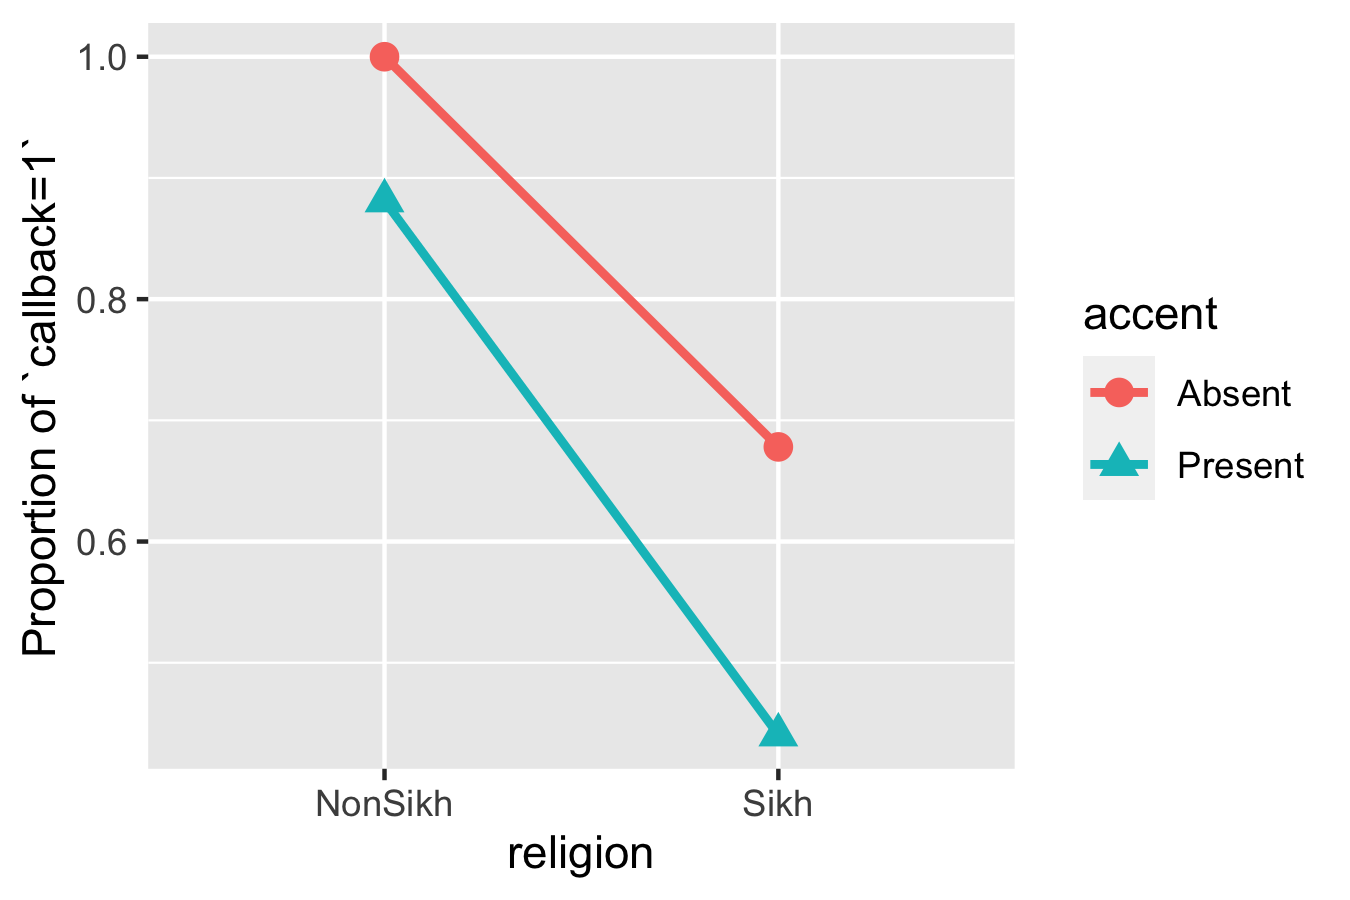
\includegraphics[width=0.65\textwidth]{../../Plots/Interaction_accent_religion.png}
    \caption{Interaction plot between \textit{religion} and \textit{accent}. Y-axis is the proportion of `\textit{callback=1}' in a group, and x-axis is the status of \textit{religion}. Color represents the status of \textit{accent}.}
    \label{fig:interact}
\end{figure}

\subsubsection{Fitting with no interaction term}
Assuming there is no detected interaction between predictors, we build the logistic regression model on response variable \textit{callback} taking four factors into account without interaction terms:
\begin{equation}
    \log \bigg(\frac{\mu_i}{1-\mu_i} \bigg) = \beta_0 + x_{i1}\beta_1 + x_{i2}\beta_2 + x_{i3}\beta_3 + x_{i4}\beta_4,\ \ \ \ i=1,2,...,n,
    \label{eq:logistic}
\end{equation}
where $i$ represents the $i^{th}$ phone message,  $\mu_i = \textnormal{E}(y_i|\mathbf{x_i}) = \textnormal{P}(y_i = 1|\mathbf{x_i})$ is the probability of $i^{th}$ phone message receives callback, $\mathbf{x_i} = [x_{i1},...,x_{i4}]$ are the values of predictors \textit{religion}, \textit{gender}, \textit{accent}  and \textit{city} for the $i^{th}$ phone message, $\beta_0$ is the intercept, and $\beta_1, ..., \beta_4$ are the regression coefficients for four predictors respectively. For  each of these binary predictors, one of the levels is taken as a baseline, and the other levels is included as a dummy variable in the model. 

A main advantage of the logistic regression model is its attractive interpretation: $\frac{\mu_i}{1-\mu_i} = \frac{P(y_i=1)}{P(y_i\neq 1)} = \frac{P(y_i=1)}{P(y_i=0)}$ can be interpreted as the \textbf{odds} of event ``$y_i=1$'', so the parameter (say) $\beta_j$ may be interpreted as the change of odds in log-scale when the $j^{th}$ predictor is changed from baseline value to alternate value. We can fit the regression coefficients in \autoref{eq:logistic} through \texttt{R}. The following presents a sample code output from applying the \texttt{glm} function on simulated data with the function parameters set to perform logistic regression:
\begin{verbatim}
> lr.fit <- glm(callback ~ religion + gender + accent + city, 
+               data = dat, family=binomial("logit"))  ## Fit the parameters
> summary(lr.fit)  ## Results summary

Call:
glm(formula = callback ~ ., family = binomial("logit"), data = dat)

Deviance Residuals: 
    Min       1Q   Median       3Q      Max  
-2.2947  -0.9460   0.2638   0.7694   1.4280  

Coefficients:
                Estimate Std. Error z value Pr(>|z|)    
(Intercept)    3.76833    0.35272  10.684  < 2e-16 ***
religionSikh  -2.70256    0.28465  -9.494  < 2e-16 ***
genderMale    -0.02224    0.21612  -0.103   0.9180    
accentPresent -1.21003    0.22274  -5.432 5.56e-08 ***
citySurrey    -0.40560    0.21796  -1.861   0.0628 .  
\end{verbatim}
From the output, the estimated intercept is 3.77 and the estimated regression slope for the four predictors are  -2.70, -0.02, -1.21, -0.41 respectively. The output gives us the fitted model:
\begin{equation}
    \begin{split}
     \log\frac{P(callback = 1|\textnormal{\textit{religion, gender, accent, city}})}{P(callback=0|\textnormal{\textit{religion, gender, accent, city}})} =\ & 3.77 -2.70*I\textnormal{(\textit{religion}=`Sikh')}  -0.02 *I\textnormal{(\textit{gender}=`male')}  \\ & -1.21*I\textnormal{(\textit{accent}=`present')}  -0.41*I\textnormal{(\textit{city}=`Surrey')},
    \end{split}
\end{equation}
where $I(\cdot)$ is the indicator function.

Take \textit{religion} for an example of interpretation. Here the baseline value is set as ``non-Sikh'' thus the alternate value is ``Sikh'' accordingly. The exponentiated estimate of coefficient for ``religionSikh'' in the \texttt{R} output, $e^{-2.70} = 0.067$, is the factor by which the odds of receiving callback is multiplied when \textit{religion} changes from ``non-Sikh'' to ``Sikh'' while other variables remain fixed. In other words, the odds of a voicemail from a Sikh person receiving callback is expected to reduce $1-0.067 = 93.3\%$ compared with a non-Sikh person. Correspondingly, we could observe from \autoref{fig:eda1}a that the callback rate in the ``Sikh'' group is notably lower than the ``non-Sikh'' group. The other three predictor coefficients can be interpreted similarly. Meanwhile, the exponentiated intercept, $e^{3.77} = 43.4$, represents the odds that a phone message receives callback when it is from a non-Sikh female with no accent in city Richmond, i.e., the baseline. 

%Meanwhile, p-values in this output, i.e. values the column $Pr(>|z|)$, are from hypothesis tests of the regression parameters $\beta_j$. In each test for $\beta_j,\ j=0,1,...,4$, the null hypothesis is $\beta_j=0$, i.e. the $j^{th}$ predictor does not have association with the log odds of ``$y_i=1$''. The p-value is the probability of obtaining test results at least as extreme as the results actually observed, under the assumption that the null hypothesis is correct. A low p-value is evidence supporting the rejection of the null hypothesis. In our case, only \textit{religion} and \textit{accent} has p-values lower than 0.05 (which is a common significance threshold in statistics). 

\subsubsection{Fitting with interaction terms}
\label{sec:logistic_interact}
If interaction effects between variables are dectected (say a 2-way interaction between \textit{religion} and \textit{accent}), we build the model with the detected interaction terms:
\begin{equation}
    \log \bigg(\frac{\mu_i}{1-\mu_i}\bigg)  = \beta_0 + \beta_1x_{i1} + \beta_2x_{i2} + \beta_3x_{i3} + \beta_4x_{i4} + \beta_5 x_{i1}x_{i3},\ \ \ \ i=1,2,...,n,
    \label{eq:logistic2}
\end{equation}
where $\beta_5$ is the regression coefficient for the interaction term, and the rest of the notations are identical with \autoref{eq:logistic}. The example \texttt{R} code is shown below:
\begin{verbatim}
> lr.fit <- glm(callback ~ religion + gender + accent + city + religion:accent, 
+               data = dat, family=binomial("logit"))  
\end{verbatim}

To be noted, adding an interaction term to a model drastically changes the interpretation of the coefficients. If there were no interaction term, $\beta_1$ would be interpreted as the unique effect of \textit{religion} on the log-odds of \textit{callback}. But the interaction means that the effect of \textit{religion} on \textit{callback} varies for different values of \textit{accent}. The unique effect of \textit{religion} is represented by everything that is multiplied by \textit{religion} in the model: $\beta_1$ + $\beta_3*I\textnormal{(\textit{accent}=`present')}$. $\beta_1$ is now interpreted as the unique effect of \textit{religion} on the log-odds of \textit{callback} only when $I\textnormal{(\textit{accent}=`present')}=0$.


\subsubsection{An alternative regression on the callback rate}

Because all explanatory variables are discrete factors, an alternative regression analysis to the logistic regression may be built on the callback rates (i.e., the proportions of ``\textit{callback}=1'') in all possible combinations of the predictors. For instance, there will be a total of 16 combinations if \textit{religion}, \textit{gender}, \textit{accent}  and \textit{city} are all included. However, rather than using the proportions directly as the response, we suggest applying a logit transformation to the callback rate so that the domain of the response is expected to be the real line rather than 0 to 1. Denoting $r$ as the callback rate, the logit transformation is given by
\begin{equation}
    \textnormal{logit}(r) = \log \bigg(\frac{r}{1-r}\bigg).
\end{equation}

An example regression equation with no interaction term would be
\begin{equation}
    \textnormal{logit}(r_j) = \beta_0 + \beta_1x_{j1} + \beta_2x_{j2} + \beta_3x_{j3} + \beta_4x_{j4},\ \ \ \ j=1,2,...,d,
\end{equation}
where $r_j$ is the callback rate from the $j^\textnormal{th}$ combination,  $\mathbf{x_i} = [x_{j1},...,x_{j4}]$ are the values of \textit{religion}, \textit{gender}, \textit{accent}  and \textit{city} from the $j^\textnormal{th}$ combination, and $\beta_1, ..., \beta_4$ are the regression coefficients. Though this regression equation looks similar to \autoref{eq:logistic}, interpretation of the coefficients is different. Here, the estimated coefficient $\beta_j$ of a predictor is interpreted as the expected difference in logit($r$) between that level of the variable and its baseline given other predictors fixed. For example, if \textit{religion} changes from ``non-Sikh'' to ``Sikh'', i.e., from baseline to the alternative level, the logit-transformed callback rate will increase a value equal to $\beta_1$. The corresponding \texttt{R} code can be found \href{https://github.com/NingShen1997/STAT551_Case34/blob/main/Code/alternative_regression.R}{here}.


\subsection{Ordinal regression on \textit{appoint\_offer}}

Instead of the odds of being one category in logistic regression, the ordinal regression model focuses on the odds of being less than or equal to a particular category. In our case, this odd is definded as $ \frac{P(Y\leq k)}{P(Y > k)}$ for $k = 0,1$ where $Y$ is the response variable \textit{appoint\_offer}, and $k$ is the category in the response. Here we won't go into the details of the case with interaction effects, but researchers shall resemble the procedure of adding interaction terms as in \autoref{sec:logit}. Here the ordinal logistic regression model is thus parameterized as
\begin{equation}
    \log \frac{P(y_i\leq k|\mathbf{x_i})}{P(y_i > k|\mathbf{x_i})} = \beta_{k0} + \beta_1x_{i1} + \beta_2x_{i2} + \beta_3x_{i3} + \beta_4x_{i4},\ \ \ \ i=1,2,...,n,\ \ \ k=0,1,
    \label{eq:ordinal}
\end{equation}
where notations are the same as \autoref{eq:logistic} except that the intercept $\beta_{k0}$ varies with category $k$. We use the \texttt{polr} function in \texttt{MASS} package from \texttt{R} to estimate the parameters in the regression model. The sample code runs as follows:
\begin{verbatim}
> or.fit <- polr(appoint_offer ~ religion + gender + accent + city, data = dat, Hess=TRUE)
> summary(or.fit)
Call:
polr(formula = appoint_offer ~ religion + gender + accent + city, 
    data = dat, Hess = TRUE)

Coefficients:
                Value Std. Error  t value
religionSikh  -3.6144     0.2379 -15.1946
genderMale    -0.3360     0.1838  -1.8281
accentPresent -2.3898     0.2131 -11.2122
citySurrey    -0.1545     0.1844  -0.8377

Intercepts:
    Value    Std. Error t value 
0|1  -5.5780   0.3543   -15.7447
1|2  -2.9841   0.2705   -11.0338
\end{verbatim}
According to the output, the estimated model can be written as:
\begin{equation}
    \begin{split}
    \log \frac{P(\textnormal{\textit{appoint\_offer}} \leq 0 |\textnormal{\textit{religion, gender, accent, city}})}{P(\textnormal{\textit{appoint\_offer}} > 0|\textnormal{\textit{religion, gender, accent, city}})}  = & -5.58 - 3.61*I\textnormal{(\textit{religion}=`Sikh')} \\ & -0.34 *I\textnormal{(\textit{gender}=`male')}   \\
    & -2.39*I\textnormal{(\textit{accent}=`present')} \\ &   -0.15*I\textnormal{(\textit{city}=`Surrey')} 
    \end{split}
\end{equation}
and 
\begin{equation}
    \begin{split}
        \log \frac{P(\textnormal{\textit{appoint\_offer}} \leq 1|\textnormal{\textit{religion, gender, accent, city}})}{P(\textnormal{\textit{appoint\_offer}} > 1|\textnormal{\textit{religion, gender, accent, city}})}  = & -2.98 - 3.61*I\textnormal{(\textit{religion}=`Sikh')} \\ & -0.34 *I\textnormal{(\textit{gender}=`male')}   \\
        & -2.39*I\textnormal{(\textit{accent}=`present')}  \\ &  -0.15*I\textnormal{(\textit{city}=`Surrey')} 
    \end{split}
\end{equation}


\begin{figure}[!t]
    \centering
    \begin{subfigure}{0.45\textwidth}
        \centering
        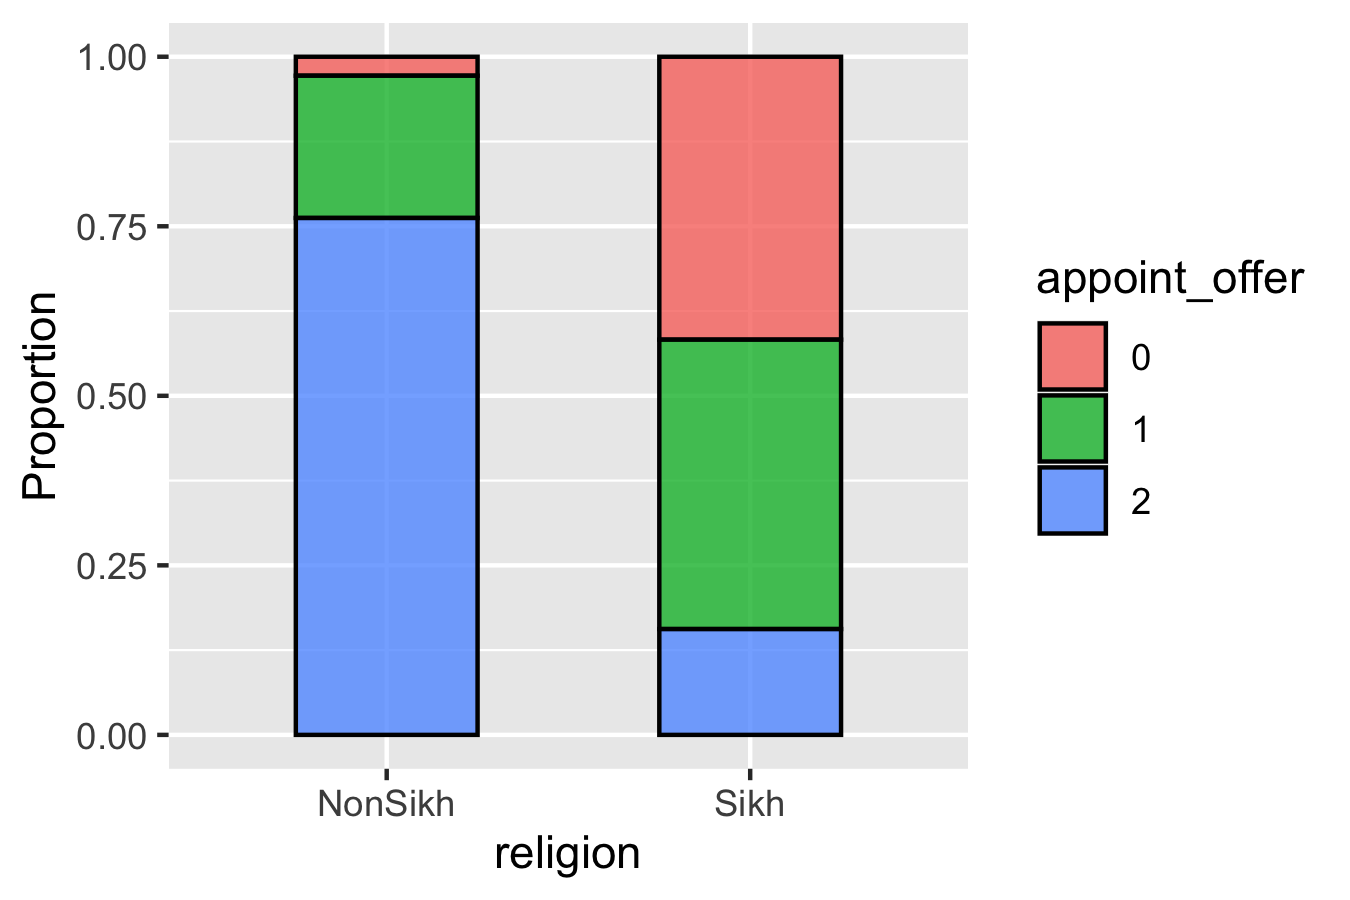
\includegraphics[width=\textwidth]{../../Plots/Proportions_appoint_offer_religion.png}
        \caption{}
    \end{subfigure}
    \begin{subfigure}{0.45\textwidth}
        \centering
        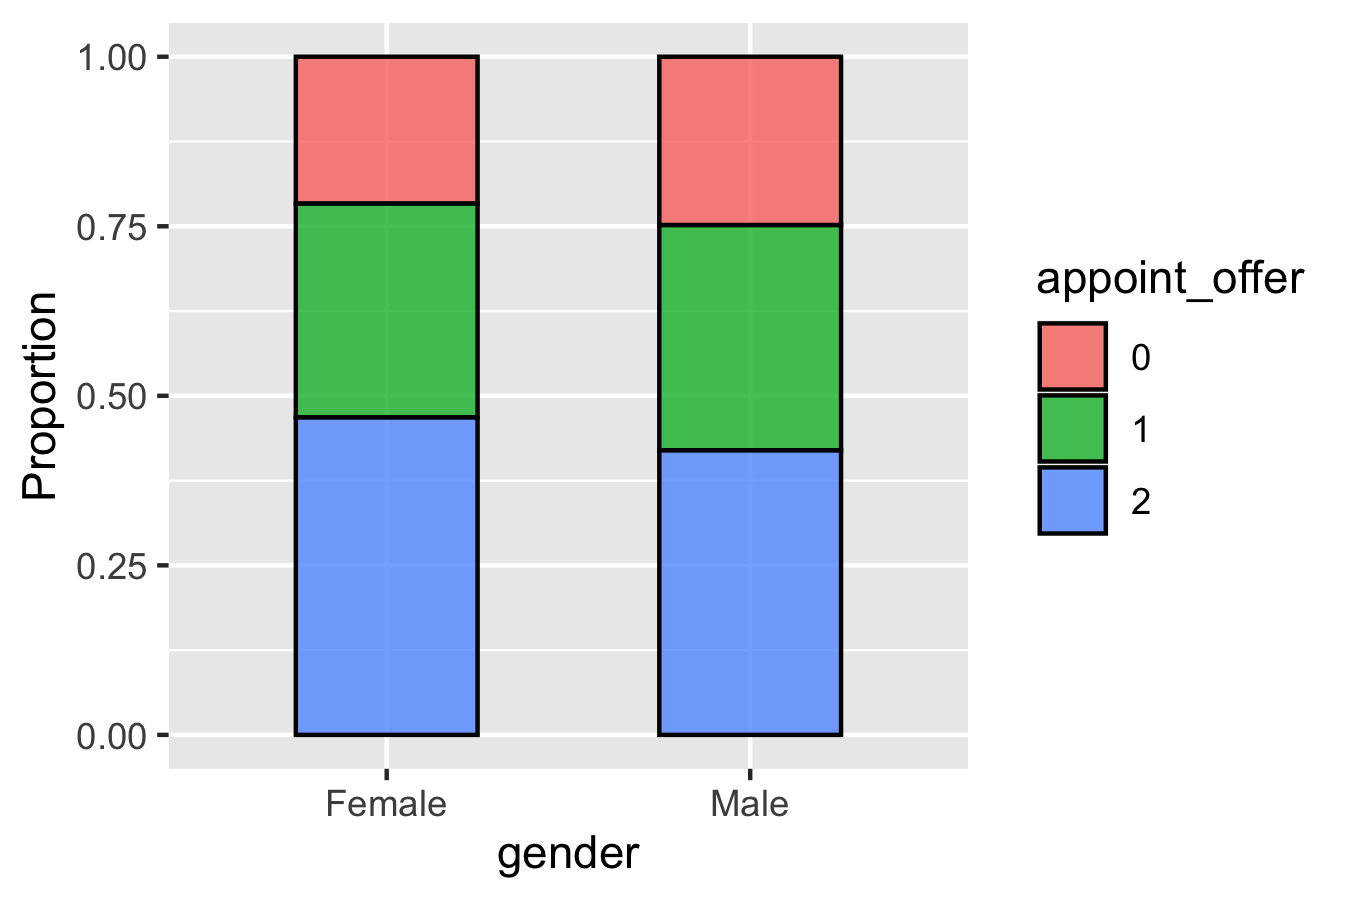
\includegraphics[width=\textwidth]{../../Plots/Proportions_appoint_offer_gender.png}
        \caption{}
    \end{subfigure}
    \begin{subfigure}{0.45\textwidth}
        \centering
        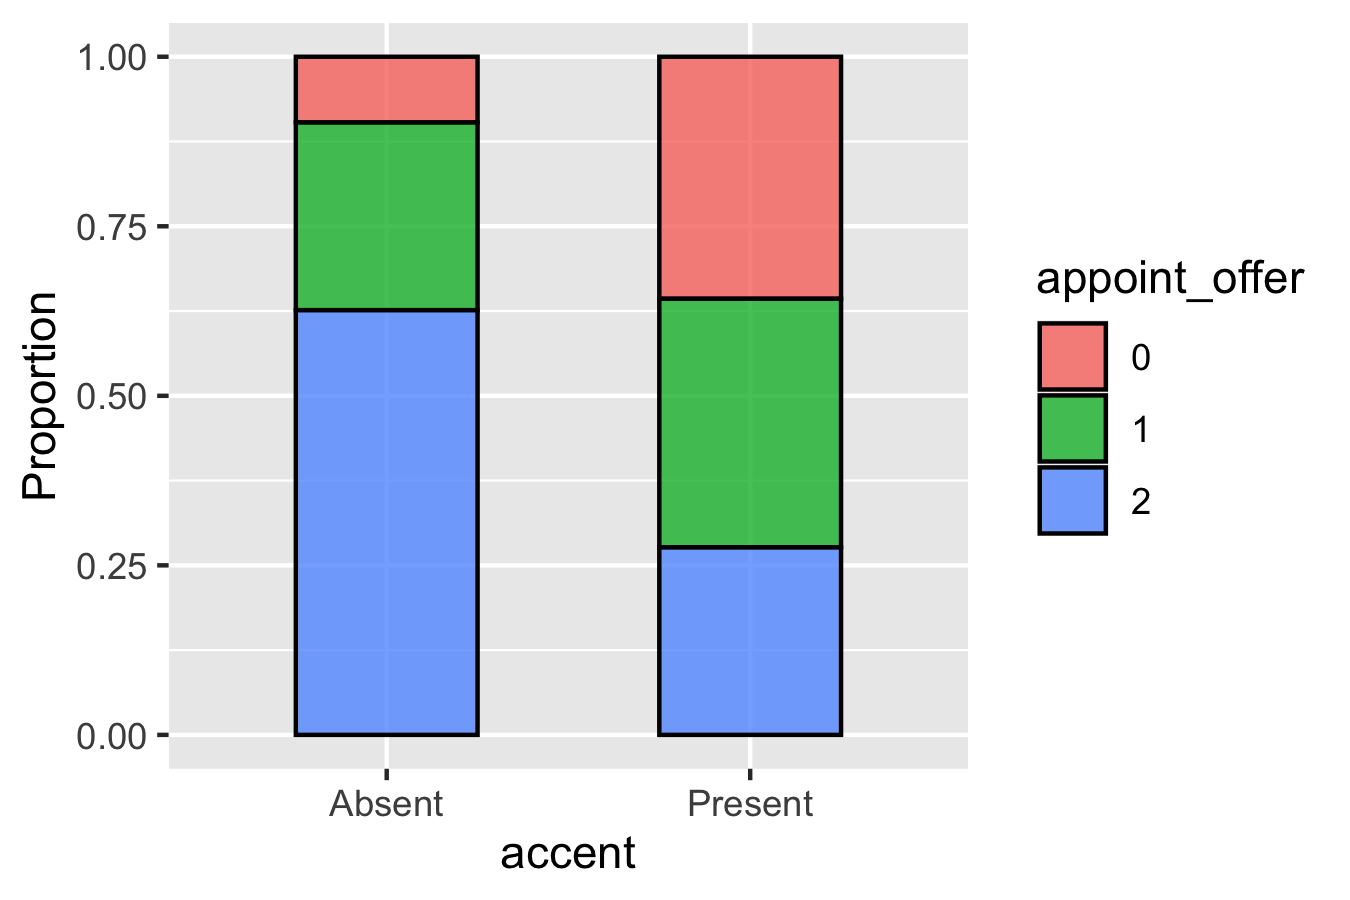
\includegraphics[width=\textwidth]{../../Plots/Proportions_appoint_offer_accent.png}
        \caption{}
    \end{subfigure}
    \begin{subfigure}{0.45\textwidth}
        \centering
        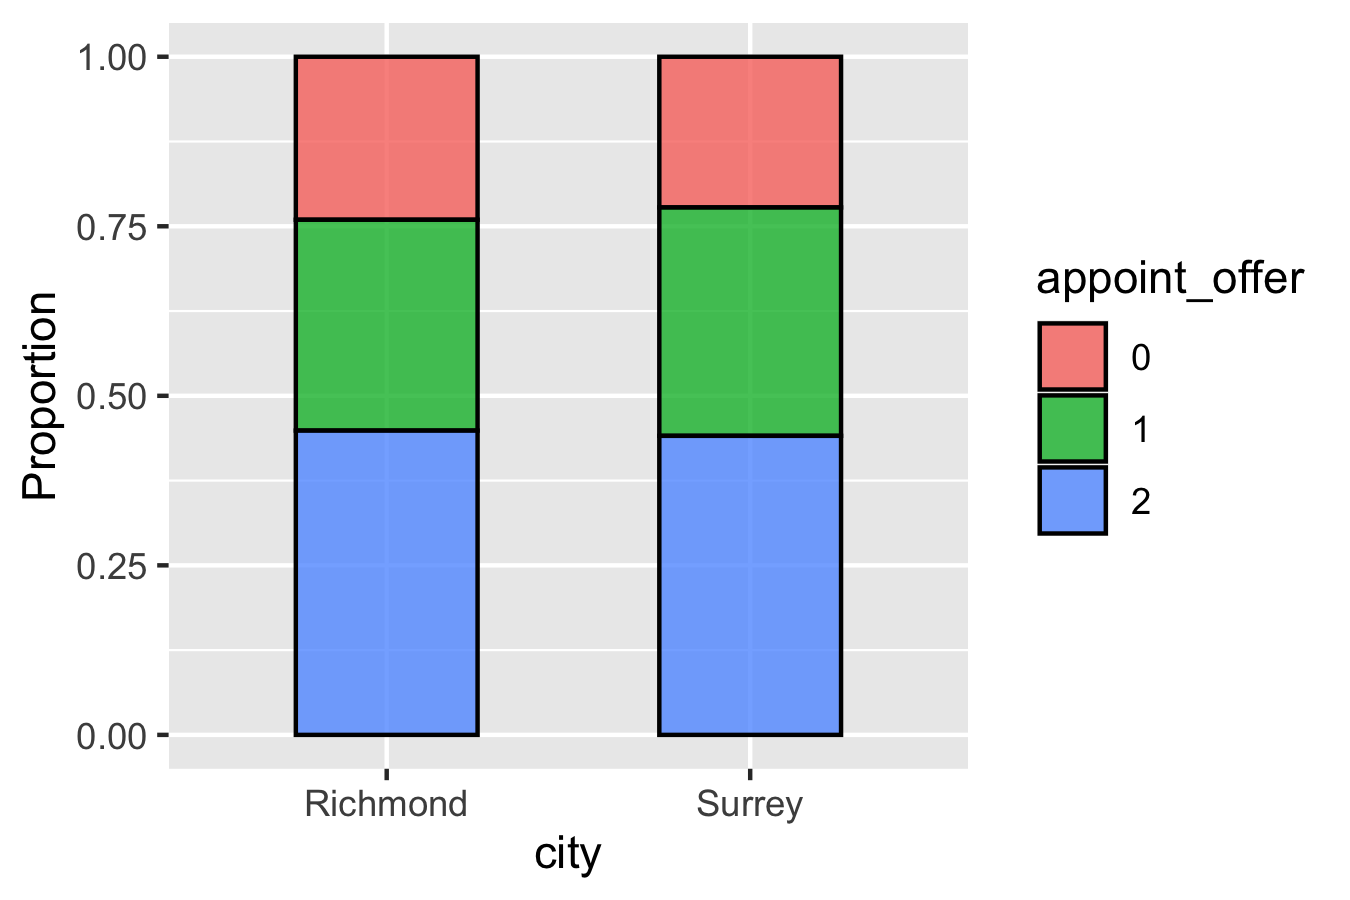
\includegraphics[width=\textwidth]{../../Plots/Proportions_appoint_offer_city.png}
        \caption{}
    \end{subfigure}
    \caption{Distribution of \textit{appoint\_offer} in predictors a) \textit{religion}, b) \textit{gender}, c) \textit{accent} and d) \textit{city}.}
    \label{fig:eda2}
\end{figure}

The estimated regression slope for the four predictors are the same for the two odds. Interpretations for the coefficients are similar to that of the logistic regression model (Eq. \ref{eq:logistic}), except for the intercepts. The exponent of first intercept $e^{-5.58} = 0.004$ represents the odds that a baseline voicemail receives ``Yes'' as the answer for requesting appointment offer. The exponent of second intercept $e^{-2.98} = 0.051$ represents the odds that a baseline voicemail receives ``Yes'' or ``Not sure'' as the answer for requesting appointment offer. In this model output, we could observe that \textit{religion} and \textit{accent} have larger influence on the possibility of receiving appointment offer, which is in accordance with \autoref{fig:eda2}. Furthermore, similar to Section \ref{sec:logistic_interact}, interaction terms shall be added to the model if they are suggested from the exploratory plots.


\section{Sample Size Calculation}
As mentioned above, a pilot experiment with 20 participants will be conducted for estimation of an appropriate sample size. A power analysis, which allows us to determine the sample size required to detect an effect of a given size with a given significance level, is included in this section. The statistical power of a hypothesis test is the probability of detecting an effect, given that there is a true effect present. On the contrary, the significance level is the probability of finding an effect that is not there. Since the main objective of the study is associated with religious disparities, we focus on predictor \textit{religion} and determine the sample size based on 2-sample comparison of proportions. There are two response variables included in the study, but for simplicity we demonstrate the analysis using \textit{callback}. The approach for power analysis introduced by \citet{wang2007} is adopted in this analysis. For programming details, please refer to my \href{https://github.com/NingShen1997/STAT551_Case34}{Github repository}.


\begin{figure}[!b] 
    \centering
    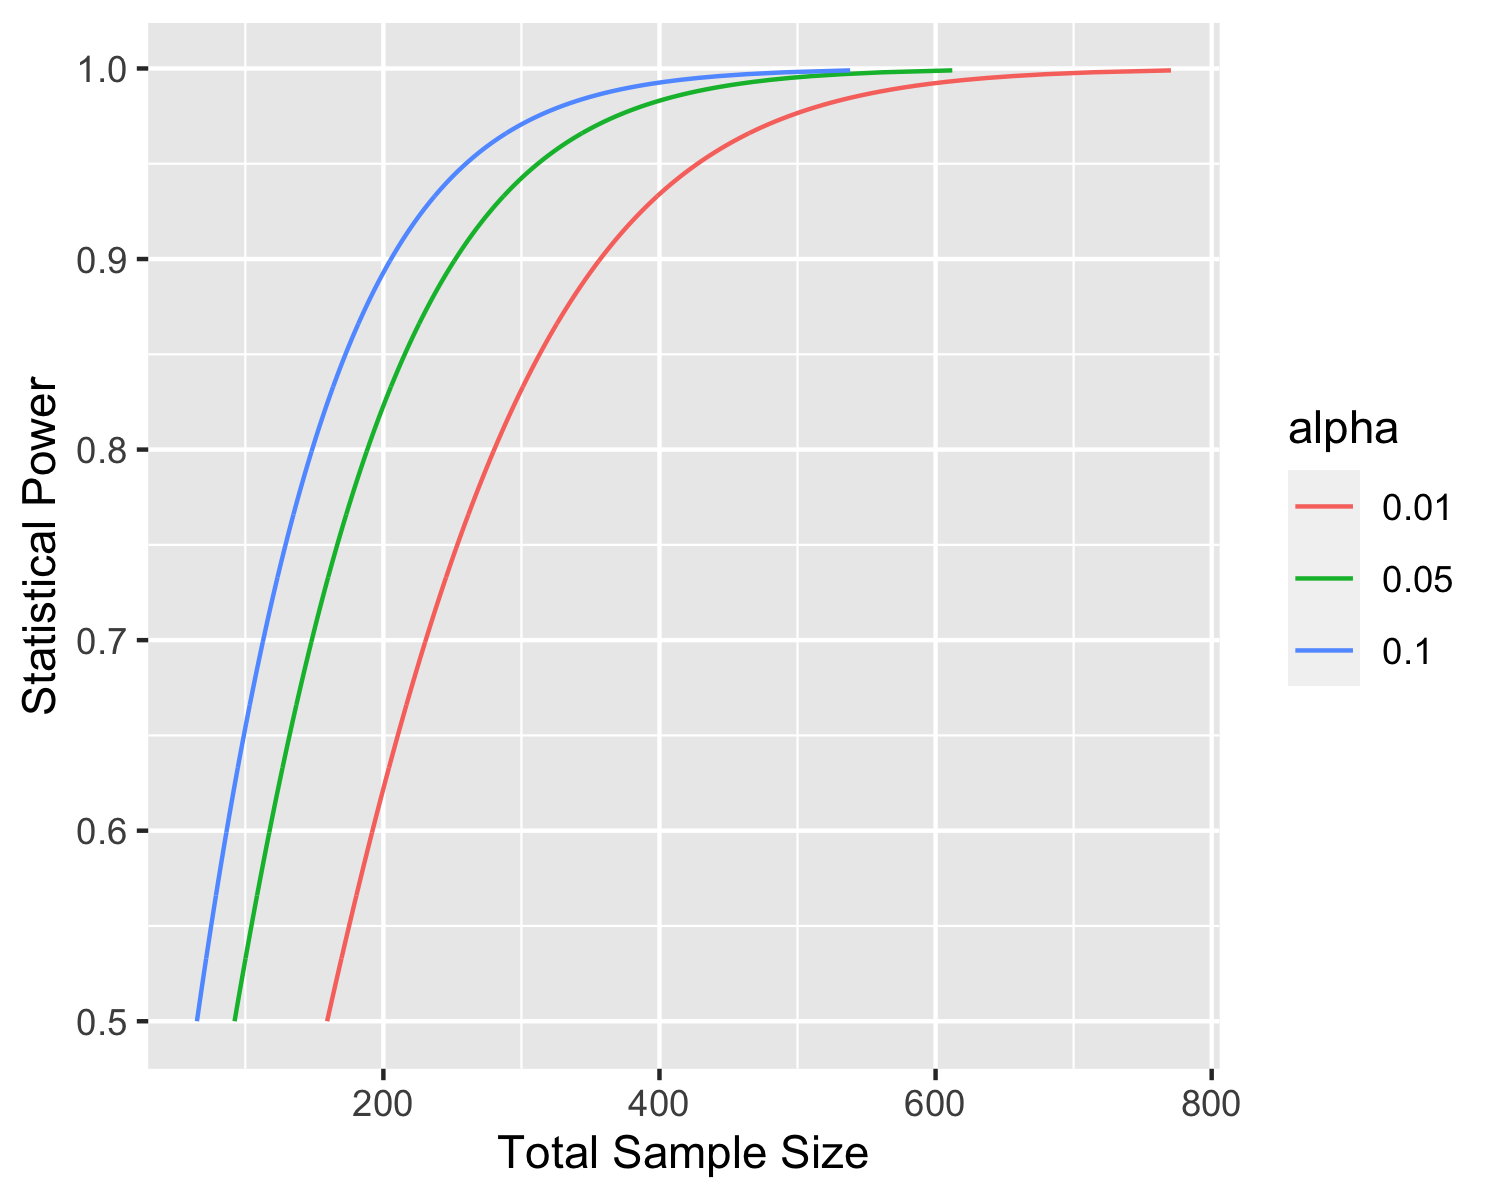
\includegraphics[width=0.8\textwidth]{../../Plots/power_analysis.png}
    \caption{Power analysis plot for 2-proportion comparison with significance level of 0.01, 0.05 and 0.1.}
    \label{fig:power_analysis}
\end{figure} 


The information that need to be gathered from the pilot experiment is the proportion of 1's in 
\textit{callback} given that \textit{religion} is `non-Sikh', $P(Y=1|X=\textnormal{`non-Sikh'}) \triangleq p_1$, and the proportion of 1's in  \textit{callback} given that \textit{religion} is `Sikh', $P(Y=1|X=\textnormal{`Sikh'}) \triangleq p_2$, where \textit{callback} is denoted as $Y$ and \textit{religion} is denoted as $X$. Then the following formula is used to calculate the total sample size $N$ for the study:
\begin{equation}
    N = 2\cdot \frac{p_1(1-p_1)+p_2(1-p_2)}{(p_1-p_2)^2} \cdot (z_{\alpha/2}+z_\beta)^2 ,
\end{equation}
where $\alpha$ is the significance level, $1-\beta$ is the statistical power, $z_{\alpha/2}$ is the critical value of the Normal distribution at $\alpha/2$ (e.g. for a confidence level of 95\%, $\alpha$ is 0.05 and the critical value is 1.96), $z_\beta$ is the critical value of the Normal distribution at $\beta$ (e.g. for a power of 80\%, $\beta$ is 0.2 and the critical value is 0.84), and $p_1$ and $p_2$ are the expected sample proportions of the two groups defined above.

\autoref{fig:power_analysis} is a power analysis plot with power calculated by the abovementioned formula. It shows the statistical power with a significance level of 0.01, 0.05 and 0.1 under sample size constraints given $p_1=0.60$, $p_2=0.40$. Sample size corresponding to different values of $p_1$ and $p_2$ can be obtained through applying the formula by researchers themselves.


\section{Conclusion}
To explore the potential bias from counsellors towards Sikh individuals at the entry point of the service, we recommend a logistic regression and an ordinal regression model to estimate the effect of factors like religion and gender on the counsellors' responsiveness and reception rate. Sample analyses for the regression models are demonstrated in the report and researchers may perform the analysis as depicted on a flexible choice of interested factors. However, the researchers should remain cautious with the factor of intergroup contact as it might be confounded with other factors such as demographic characteristics of the counsellor. An example power analysis for the sample size determination is also presented. 

\clearpage
\appendix
\counterwithin{figure}{section}

\section{Figures}
\setcounter{figure}{0} 
\begin{figure}[!h]
    \centering
    \begin{subfigure}{0.45\textwidth}
        \centering
        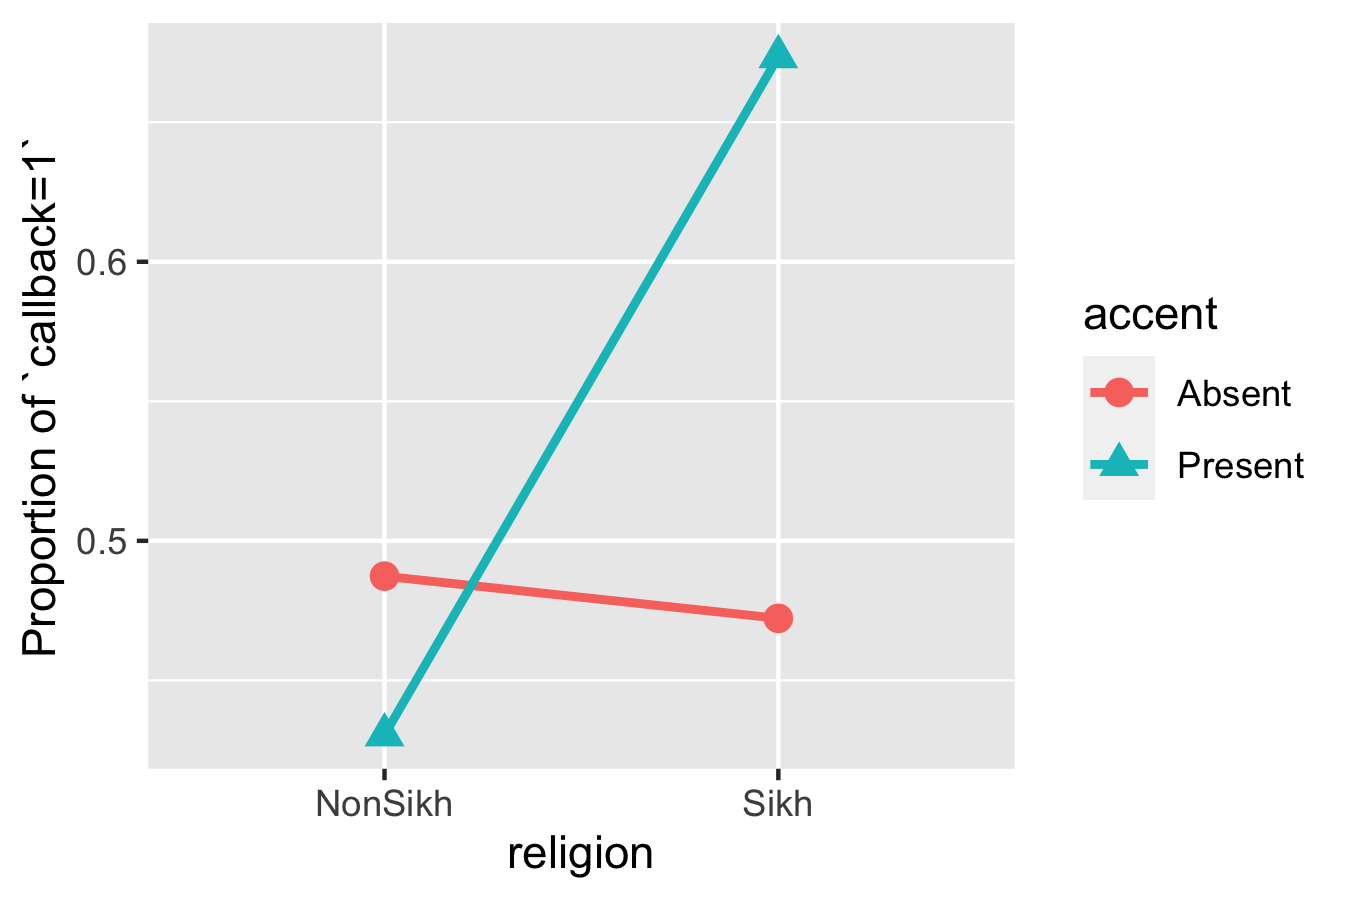
\includegraphics[width=\textwidth]{../../Plots/Interaction_accent_religion_negative.png}
    \end{subfigure}
    \begin{subfigure}{0.45\textwidth}
        \centering
        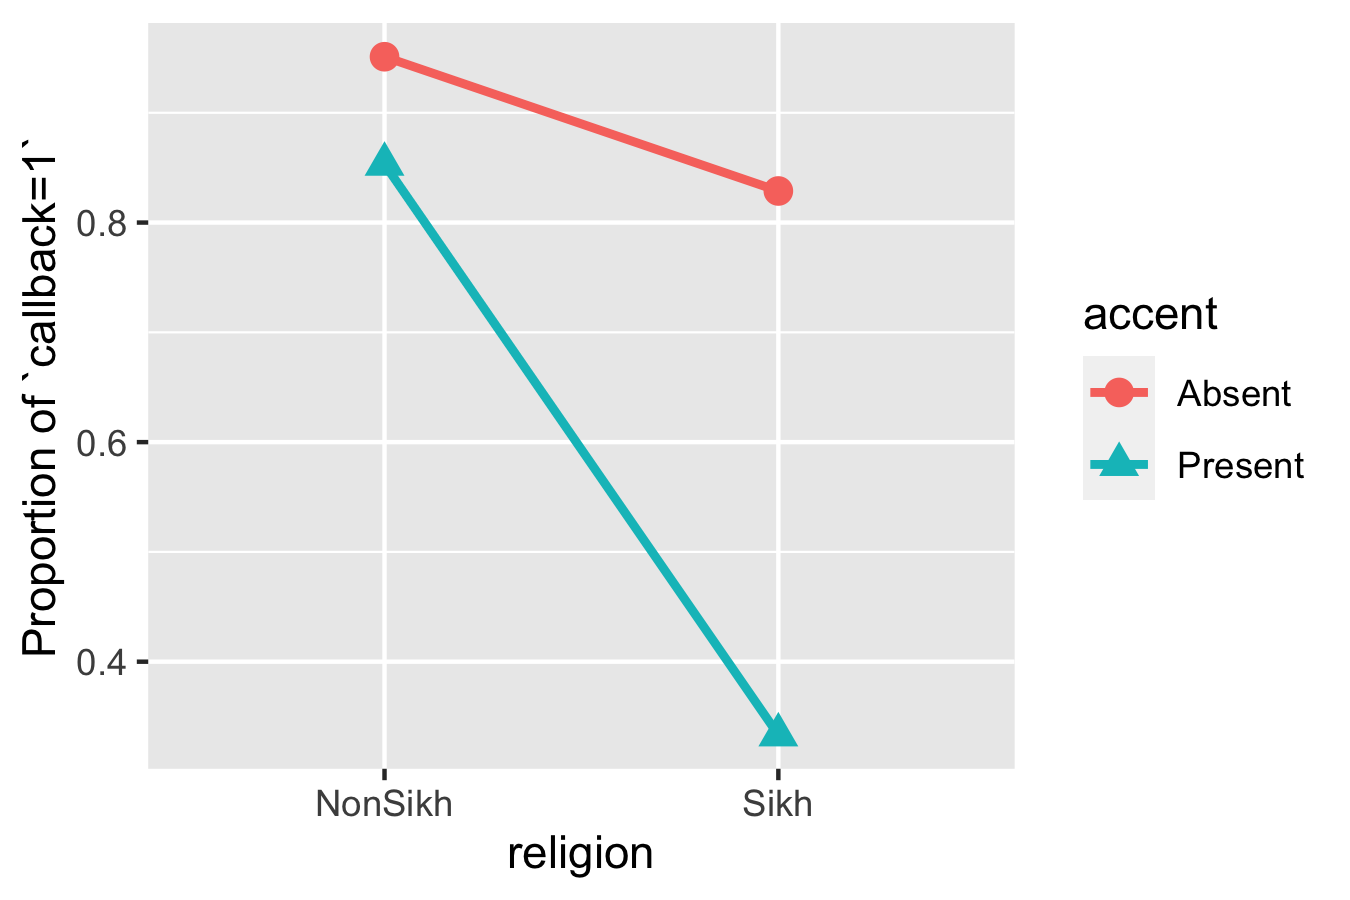
\includegraphics[width=\textwidth]{../../Plots/Interaction_accent_religion_positive.png}
    \end{subfigure}
    \caption{Examples of interaction plot between \textit{religion} and \textit{accent} with interaction present. Y-axis is the proportion of `\textit{callback=1}' in a group, and x-axis is the status of \textit{religion}. Color represents the status of \textit{accent}.}
    \label{fig:interact2}
\end{figure}

\clearpage
\begin{singlespace}
\raggedright
%\bibliographystyle{apalike}
\bibliography{bib}
\end{singlespace}

\end{document}



